\section{Introduction}

Agentic workflows based on artificial intelligence (AI) are quickly
revolutionizing high-performance computing (HPC), making it possible for
machine learning algorithms to control the flow of HPC workflows and allowing
them to be more accurate and/or flexible. In a standard HPC workflow, a series
of program-defined computational phases (modeling, simulation, analysis,
visualization, etc.) ingest and produce data toward an end scientific result.
An agentic workflow, by contrast, is a computational workflow in which one or
more AI agents---software components that use AI to make independent decisions
on behalf of users---observe intermediate data results during execution and
dynamically select the next phase(s). Agentic workflows have proven beneficial
in various scientific fields, such as molecular dynamics, alloy discovery, and
computational chemistry. For instance, agents that selectively prune data to
limit simulation to high-potential pathways (protein configurations, material
models, etc.) lead to significant performance gains, such as in DeepDriveMD,
where performance improved by $2.33\times$. Other agentic workflows increase
the flexibility of HPC workflows, allowing them to leverage out-of-domain
knowledge to automate processes previously limited to human experts, such as
metallic alloy design.

% DECLARED HERE ON PURPOSE -- TARGET IS THE TOP OF COLUMN 2, PAGE 1.
% A float goes to the top of the first column built AFTER its declaration, so
% declaring it before any body text put it at the top of column 1 and pushed
% the abstract down. Column 1 holds the abstract plus roughly the first two
% paragraphs, so declaring it here sends it to column 2 instead.
%
% THIS IS THE KNOB. Moved one paragraph EARLIER on 2026-08-10: with the
% abstract drafted, column 1 holds abstract + index terms + roughly the first
% paragraph only, so declaring after paragraph 2 was past the end of column 2
% and the float fell to page 2. If it now lands in column 1, move it one
% paragraph later; if it slips to page 2 again, one earlier. Re-check whenever
% the abstract's length changes -- the abstract is what sets where column 1
% ends.
\begin{figure}[tb]
\centering
% PLOT SPEC (kept for provenance; rendered by
% scripts/figures/make_figures.py -> figure_drafts/fig-intro-behavior.pdf)
%   two stacked timelines. Top: a traditional HPC workflow, phases with
%   declared inputs, staging bars for phase $n{+}1$ overlapping computation
%   of phase $n$, no exposed stall. Bottom: an agentic workflow, where the
%   data need for phase $n{+}1$ becomes visible only after the agent's
%   decision point, so the staging bar starts late and a stall band is
%   exposed. Mark the agent decision points explicitly --- the late arrival
%   of the need is the whole figure.
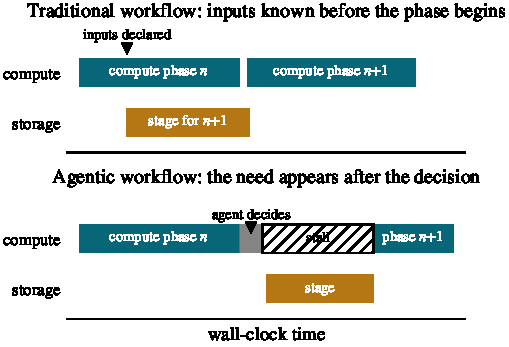
\includegraphics[width=\columnwidth]{figures/fig-intro-behavior}
\caption{Phase-based staging works when the data need is known before the
phase begins, and fails when it appears only after a steering decision---too
late to hide the transfer.}
\label{fig:intro-behavior}
\end{figure}

However, agentic workflows fundamentally challenge several key assumptions on
which existing memory and storage management in high-performance computing
systems are based. In particular, workflow phases are expected to proceed
synchronously, reuse predictable data, and have one source of direction or
control. This poses a problem because scientific simulations ingest and
produce large amounts of data---sometimes more than $O(100$~TB$)$---and
therefore cannot feasibly hold all the data required for the workflow in CPU
RAM or GPU VRAM at once, depending on the compute step. This manifestation of
the infamous ``memory wall'' problem results in longer overall wall time for
workflow executions and processing-unit idle time, during which processing
units incur energy and financial costs while performing no simulation work.
Simply adding DRAM is a costly measure that does not scale easily across
scientific workflows. Traditional HPC workflows could have their data needs
fully predicted by inserting ``hints'' into the workflow's source code.
Agentic workflows have no such---or highly limited---source code because
decisions that would have been defined in the program's flow of control are
instead made at runtime. Not only does this revive the memory-wall problem
faced by all HPC workflows, but the various specialized LLMs backing different
agents within a workflow add further memory pressure, since the parameters for
each model can occupy hundreds of gigabytes.

In traditional HPC workflows, prior solutions leveraged predictable
phase-based execution to expose a unified memory-and-storage hierarchy to the
workflow, prefetching relevant data from storage and placing it in memory
before the phase in which it was needed. Overlapping data movement for the
next phase with computation in the current phase allowed storage to be used as
an extension of memory for data-intensive workflows without exposing the
overheads of storage access. This ``Deep Memory and Storage Hierarchy'' (DMSH)
could be presented to applications as a massive memory pool without incurring
significant performance penalties. As illustrated in
Figure~\ref{fig:intro-behavior}, this approach has worked for traditional HPC
workflows because each phase has known inputs and outputs. The required data
is therefore known before each phase begins, allowing retrieval to overlap
with computation in the preceding phase. In agentic workflows, the inputs for
a given phase---or even the ordering of the phases themselves---are not
available until a steering model produces control decisions, which may be
delayed, incrementally produced, and sporadic.

This means prior work that uses storage to extend memory for non-agentic HPC
workflows cannot prefetch the correct data for each step in agentic HPC
workflows. These systems must rely on deterministic data-selection policies
designed for non-AI-steered workflows. On our tested workloads, every stall
these systems incur occurs because the staging window is too small to hide the
transfer: the data need becomes visible only after the agent has committed to
it. Agentic workflows consequently stall while the required data is fetched
from storage into memory. Incorrectly prefetched data also pollutes the memory
cache when it is read but not used in the next workflow phase. The result is
that a state-of-the-art DMSH system increases end-to-end wall time by
$3.2\times$ on our workloads rather than decreasing it as it does for
traditional workflows.

Because DMSH solutions are not broadly applicable here, these performance
losses become economic and sustainability costs. Idle accelerators and
unnecessary transfers consume power and allocation on systems that are already
constrained, and the usual escape---provisioning more DRAM or bandwidth---is
least available to the institutions running fixed on-premise infrastructure or
handling data that cannot leave it. Efficient data movement is therefore a
first-order concern for making agentic workflows viable at all, not a
secondary optimization.

Designing a memory and storage management system that enables efficient
agentic HPC workflows requires addressing several challenges. First, most of
the cost of making scientific data usable is not byte movement: in the
artifact we decompose directly, 93.0\% of the cost is representation change
performed inside the consumer process, and no amount of correctly placed bytes
removes it. Second, transformed scientific data structures and the parked
weights of the models backing the agents are both anonymous process memory
drawn from a single allocation, so they compete directly. A gigabyte of
retained memory is not uniformly valuable, with the seconds of stall avoided
per gigabyte retained spanning $65\times$ across representations. Third,
information about what the workflow will need next is available only at coarse
and fine granularities that are individually insufficient and remain imperfect
in aggregate. Speculative work must therefore be bounded so that an incorrect
prediction cannot destroy a correct retention decision.

To address these challenges, we propose \sysname, a middleware runtime that
manages a host-memory budget shared by the models backing an agentic workflow
and the scientific data consumed by its tools. \sysname{} contains (1) a
retention arbitrator that decides which models and transformed data structures
remain resident between uses and (2) an opportunistic prefetcher that stages
resources ahead of need using memory that the arbitrator has not claimed.

The retention arbitrator treats residency as a budgeted choice rather than a
fixed priority across classes. Both classes can be held in a state that makes
the next use nearly free: parking a model's weights in host memory turns a
782~s cold start into a 2.1~s wake, and retaining a parsed artifact in a live
worker turns 93.7~s of reconstruction into 10.6~s. They draw on one
allocation, and neither can be surrendered in part, so the arbitrator ranks by
stall avoided per gigabyte held---discounted by time to next use---and solves
for the best subset that fits rather than evicting one victim at a time.

The opportunistic prefetcher supplies what retention structurally cannot: a
first use has nothing to retain. It stages only into memory the arbitrator has
left unclaimed, taking horizons from a predictor that merges a planner's
declared sequence with learned tool-to-tool succession. That restriction is
what makes speculation pay at realistic prediction quality. Swept across
horizon accuracies from 0.15 to 1.00, slack staging never turns negative,
improving on the recency-ranked baseline by 5.7--18.7\%, while the same
mechanism permitted to displace a resident swings to $-6.2$\% at the low end.
And where the budget is large enough that no eviction ever occurs---so the
arbitrator is provably idle---staging alone still accounts for an 11.9-point
margin.

We evaluate \sysname{} on workflows built with the AtomAgents framework,
reporting stall and end-to-end wall time, isolating each mechanism's
contribution, measuring the CPU cost resident workers impose on foreground
agent work, and characterizing sensitivity to the planning horizon,
accelerator topology, and predictor accuracy. We compare against a runtime
that retains nothing and a recency-ranked policy that already retains both
resource classes. We report against both throughout,
because retention alone is obtainable from an inference server and a
persistent worker process; what the recency-ranked baseline lacks is
value-aware arbitration.

\medskip
\noindent The main contributions of our paper include:

\begin{itemize}

\item We show that the phase-predictability assumption behind deep memory and
storage hierarchy (DMSH) systems fails under AI-driven control, and that byte
placement is the wrong unit of work regardless: 93.0\% of the cost of making a
scientific artifact usable is representation change inside the consumer
process, and a gigabyte of retained memory varies $65\times$ in value across
representations.

\item We present \sysname, a middleware runtime managing agent-backing models
and transformed scientific data against a single host-memory budget. A
retention arbitrator treats residency as subset selection, ranking candidates
by stall avoided per gigabyte held and discounting by time to next use; a
subordinate prefetcher stages into unclaimed memory, displacing a resident
only under strict conditions.

\item We show \sysname{} reduces stall and end-to-end wall time by
34.5--50.8\% against a runtime that retains nothing, and by a further
10.3--17.1\% against a recency-ranked baseline that already retains both
classes. We attribute the gain per mechanism and report where each stops:
retention cannot help a first use, staging cannot help without a window, and
above roughly 86\% of the footprint neither is needed.

\end{itemize}
